\documentclass{article}
 
\usepackage{arxiv}

\usepackage[utf8]{inputenc} % allow utf-8 input
\usepackage[T1]{fontenc}    % use 8-bit T1 fonts
\usepackage{hyperref}       % hyperlinks
\usepackage{url}            % simple URL typesetting
\usepackage{booktabs}       % professional-quality tables
\usepackage{amsfonts}       % blackboard math symbols
\usepackage{nicefrac}       % compact symbols for 1/2, etc.e
\usepackage{microtype}      % microtypography
\usepackage{lipsum}		% Can be removed after putting your text content
\usepackage{graphicx}
\usepackage{natbib}
\usepackage{hyperref}
\usepackage{multicol}
\usepackage{caption} 
\usepackage{float}
\captionsetup[table]{skip=10pt}
\captionsetup[table]{skip=10pt}

\hypersetup{
    colorlinks=true,
    linkcolor=blue,
    filecolor=blue,      
    urlcolor=blue,
    pdftitle={Overleaf Example},
    pdfpagemode=FullScreen,
    }
    
\title{Lightweight Activity Recognition for Autism Diagnosis}

\author{Anish Lakkapragada \\
	Lynbrook High School\\
	San Jose, CA 95129 \\
	\texttt{anish.lakkapragada@gmail.com} \\
	%% examples of more authors
	\And
	Peter Washington \\
	Stanford University \\ 
	Stanford, CA 94305 \\
	\texttt{peter100@stanford.edu} \\
	
	\And
	Dennis Wall \\
	Stanford University \\ 
	Stanford, CA 94305 \\
	\texttt{dpwall@stanford.edu} \\
}


%\renewcommand{\headeright}{Technical Report}
%\renewcommand{\undertitle}{Technical Report}


\begin{document}
\maketitle

\begin{abstract}
	\emph{A formal Autism Spectrum Disorder (ASD) diagnosis is an inefficient and lengthy process. Families often have to wait a few years before receiving a formal diagnosis for their child; some even may not receive one at all. One approach to this problem is to use digital technologies to detect presence of behaviors related to ASD, which in aggregate may lead to remote and automated diagnostics. One of the strongest indicators of ASD is stimming, which are repetitive, self-stimulatory behaviors such as hand flapping, headbanging, and spinning. However, using computer vision to detect such behaviors is especially difficult due to the sparsity of training data and excessive shakiness and motion. Our work demonstrates a method for addressing this problem: we employ hand landmark detection over time as a feature representation which is then fed into a Long Short-Term Memory (LSTM) model. We achieve blank validation accuracy and a blank F1 score on detecting whether videos from the Self-Stimulatory Behaviour Dataset (SSBD) contain hand flapping or not. Our model also uses less than blank parameters, providing promise for deployment into a ubiquitous and wearable digital settings for remote ASD diagnosis. }
\end{abstract}


\section{Introduction}

Autism Spectrum Disorder (ASD) affects almost 1 in 40 people in America \cite{kogan2018prevalence} and is the fastest growing serious developmental disability in the United States \cite{ardhanareeswaran2015introduction, gordon2016whittling}. Despite the fact that by 24 months of age autism can be diagnosed accurately \cite{lord2006autism, sacrey2015early}, the average age of diagnosis is typically from 3.5 to 5 years \cite{committee2013pediatrician}. This problem is further exacerbated by the fact that better treatment outcomes happen with earlier intervention \cite{estes2015long}. 

To solve this problem, we believe that the usage of some sort of mobile app with deep learning models will help ASD diagnosis be done quicker with just the same accuracy. Today’s typical ASD diagnosis doesn’t rely heavily on biometric information or tests; instead it relies more on observation of the child’s behavior. Aside from repetitive behaviors like hand flapping, a lot of the behaviors and tendencies prevalent in those with ASD such as gaze patterns and facial expressions can be reliably detected with the use of machine learning. We will explore the literature of using machine learning in ASD deeper in our Related Work section. 

One of the strongest indicators of ASD used in diagnosis is stimming, or repetitive, self-stimulatory behaviors like hand flapping, headbanging, and spinning. Using deep learning for detection of these behaviors specifically is difficult due to the lack of video data; whatever videos exist often are recorded on a handheld camera so they may be shaky or unstable. In our work we demonstrate how it is possible for this problem to be alleviated with our landmark detection approach.

Landmark detection is an active field of computer vision that detects the various landmarks on somebody’s body. Such software is usually optimized to detect landmarks on a specific body part, like the face or hands and will return the positions/coordinates of where those landmarks are in the image. 

Our method takes a set of 90 frames of a given video, and for each frame performs hand landmark detection to identify the positions of a set amount of landmarks on any hands shown. The coordinates of all of these landmarks are concatenated to make one vector which is then fed into a Long-Short Term Memory (LSTM) model \cite{hochreiter1997long} (for each frame). We call this vector the "location frame", because it gives us the locations of the hands in a single frame. We achieve blank validation accuracy with this method. This approach gives us results and is extremely light, which makes it suitable for deployment in mobile apps to increase diagnosis outreach. We will describe our data processing and methods in greater detail later. 

\section{Related Work}

Before we go over that though, we would like to go over how deep learning has already been used towards ASD diagnosis. Because there no single approach or indicator in ASD diagnosis, it follows that there will be a myriad of diverse methods towards using machine learning to detect autism. 

\subsection{Gaze Patterns}
Chang et. al found a statistically significant difference that those with ASD would spend more time looking at a distracting toy than a person engaging in social behavior in a movie when compared to those with typical development (TD) \cite{PMID:33900383}. This proves that gaze patterns and a preference to social stimuli is a good indicator of ASD. Gaze patterns have been applied as features in machine learning classifiers. Jiang et al. created a random forest classifier that took in a subject’s performance in classifying the emotion shown in a photo and other features about their gaze and face \cite{8857005}. They achieved 86\% accuracy with this approach on classifying autism.  Liaquat et. al used convolutional neural networks (CNNs) \cite{lecun1989backpropagation} and LSTMs on a public gaze dataset and achieved 60\% accuracy on the test set \cite{LIAQAT2021116198}. 

\subsection{Facial Expression}
Another approach towards autism detection is facial expression. Those with ASD usually have a different facial expression than those who are NT for the same emotion. This was found by Volker et al. \cite{FacialEncodingForHFASD} who discovered that NT raters had a harder time recognizing sadness in the facial expressions of those with autism than controls. This research was validated by Guha et al., who found that those with autism typically had less facial symmetry \cite{7178080}. A good example of how this feature can be used in deep learning is demonstrated by Li et al., who achieved an F1 score of 76\% by using a CNN to extract features of facial expressions in an image and then utilizing these features to classify autism \cite{8803604}. CNNs, along with Recurrent Neural Networks (RNNs) \cite{rumelhart1985learning}, were also applied in Zunino et al.'s work where videos were used to classify autism \cite{8545095}. They achieved 72\% accuracy on classifying those with autism and 77\% accuracy on classifying those with TD. 

\subsection{On-Body Devices} 

Smartwatch-based systems and sensors have been used in research to detect repetitive behaviors to help with intervention for those with autism. Westeyn et al. used a Hidden Markov model to detect stimming based on accelerometer data of 7 different types of self-stimulatory behaviors \cite{westeyn2005recognizing}. They achieved 69\% accuracy with this approach.Albinali et al. tried using accelerometors on the wrists and torsos to detect stimming in those with ASD \cite{albinali2009recognizing}. They achieved an accuracy of 88.6\%. Sarker et. al used a commercially available smartwatch to collect data of adults performing stimming behaviors like headbanging, hand flapping, and repetitive dropping \cite{sarker2018detection}. The smartwatch also had a 3-axis accelerometer and 3-axis gyroscope. They used 70 features from the accelerometer and gyroscope data to build a gradient boosting based model with an accuracy of 92.6\% and an F1 score of 88.1\%. However, it is important to note that while these techniques may have yielded high accuracy they may not be the best for an accessible, high-outreach autism diagnosis. 

\subsection{Pose Estimation}
The last approach we would like to go over is the usage of pose estimation and activity recognition in detection of self-stimulatory behaviors, as it is the closest method to this work. Vyas et al. retrained a 2D Mask R-CNN \cite{girdhar2018detecttrack} to get the coordinates of 15 keypoints that were then transformed into a Pose Motion (PoTion) representation \cite{8578832} and finally fed to a CNN model for a prediction on whether there was ASD-related behavior in the video \cite{8918863}. This gave a 72.4\% classification accuracy with 72\% precision and 92\% recall. We note however that they used a derived 8349 episodes from private videos of the Behavior Imaging company to train their model. Rajagopalan et al. used the Histogram of Dominant Motions (HDM) from a video, which gives the dominant motions detected, to train a discriminatory model to detect self-stimulatory behaviors \cite{7025294}. On the Self-Stimulatory Behavior Dataset (SSBD) \cite{6755972}, that we also use in this work, they accomplished 86.6\% accuracy on detecting headbanging or spinning behavior and 76.3\% accuracy on detecting headbanging, spinning, or hand flapping behavior. We note that they didn't train a classifier with a control class. 

\subsection{A Note about Efficiency}
To the best of our knowledge, we are the first ones to use just the coordinates of (hand) landmarks as features to a single model to detect hand flapping. Because one of our biggest goals is using machine learning classifiers in apps and other accessible services for a faster ASD diagnosis, in contrast to previous works we strive to make our models and feature representations as light as possible. 

\section{Data}

\subsection{Dataset}

For our work, we use the Self-Stimulatory Behavior Dataset (SSBD) \cite{6755972}. To the best of our knowledge, it is the only publicly available dataset we can find that gives access to videos of self-stimulatory behaviors, more specifically headbanging, hand flapping, and spinning, being performed. In more detail, SSBD gives you the URLs of 75 YouTube videos and for each video the time section(s) (e.x. second 1 to second 35) of when a certain self-stimulatory behavior was performed. There might be more than one time section in a single video for the same behavior (e.x. seconds 1 to 3 and 5 to 9 both have hand flapping), or there could be different behaviors performed in the same video at different sections (e.x. seconds 1 to 3 show headbanging and seconds 5 to 9 show hand flapping.) 

\subsection{Data Preprocessing}

Because our objective was to train a classifier to detect hand flapping in a video, aside from hand flapping videos we would need control videos (with no hand flapping.) To do this, we first downloaded all of the YouTube videos that had sections of hand flapping. Then, in a given video the sections of hand flapping would be cut out to make a new video. Parts of the video where there was no hand flapping (i.e. the lack of being in an annotated section) would be cut out to make control videos. Our process to create positive and control videos from a single video is illustrated in Figure 1. 

\begin{figure}[h!]
\centering
\includegraphics[scale=0.5]{figures/DataPreprocessing.png}
\caption{Illustration of our process to create positive and control videos. In the above video, sections of hand flapping on the leftmost and rightmost of the figure will be used to create positive videos, and the segment in the middle will be used to create control videos.}
\label{fig:method}
\end{figure}

Even after extracting all positive and control videos from the downloaded videos, we still wanted to maximize the amount of training data we had. Because it only takes a few seconds to recognize the presence or absence of hand flapping if a video is greater than 2 seconds we would cut it up to create more positive and control videos. Because a lot of the YouTube videos were recorded on a handheld camera, some of them would be shaky or low-quality, so we manually went through the videos to only keep high-quality data. We also noticed that a lot of the videos were of children only, so we recorded 3 control videos and 3 positive videos of ourselves to see whether a model could generalize past age (and hand shape.)  \footnote{The dataset is uploaded to google drive \href{https://tinyurl.com/47fya6}{here}.}

\section{Method}
\subsection{Approach} 

When designing a model that we assume to be used on a mobile device, as said before the first constraint is size; a higher accuracy doesn't change the fact that heavy models will not be able to fit on a model. With that in mind, we try to engineer a feature representation that will not only be light but also not need heavier models, like CNNs. Instead of using a pose estimation image for each frame that will need to be fed into a Time-Distributed CNN and then an RNN, we use the numerical coordinates of the detected hand landmarks.

To do this, we use MediaPipe, a framework by Google that can be used to detect the landmarks on a person's face, hands, and body in a given image \cite{lugaresi2019mediapipe}. MediaPipe's hand landmark detection model gives the \emph{(x, y, z)} coordinates of each of the 21 landmarks it detects on a hand. The \emph{x} coordinate and \emph{y} coordinate gives how far the landmark is on the horizontal and vertical dimension respectively. The \emph{z} coordinate gives approximately how far the landmark is from the camera. Both the \emph{x}, \emph{y}, and \emph{z} coordinates all are on a scale of approximately 0 to 1. In the case that mediapipe doesn't detect a landmark, we set the \emph{(x, y, z)} coordinates all to 0. Figure 2(a) shows the 21 landmark MediaPipe detects (as shown in documentation), and Figure 2(b) shows MediaPipe's detected hand landmarks drawn on a hand. Please note that it is the points in the figures that are the landmarks; the green lines are only there to make the hand shape more obvious. 

\begin{figure}%
    \centering
    (a){{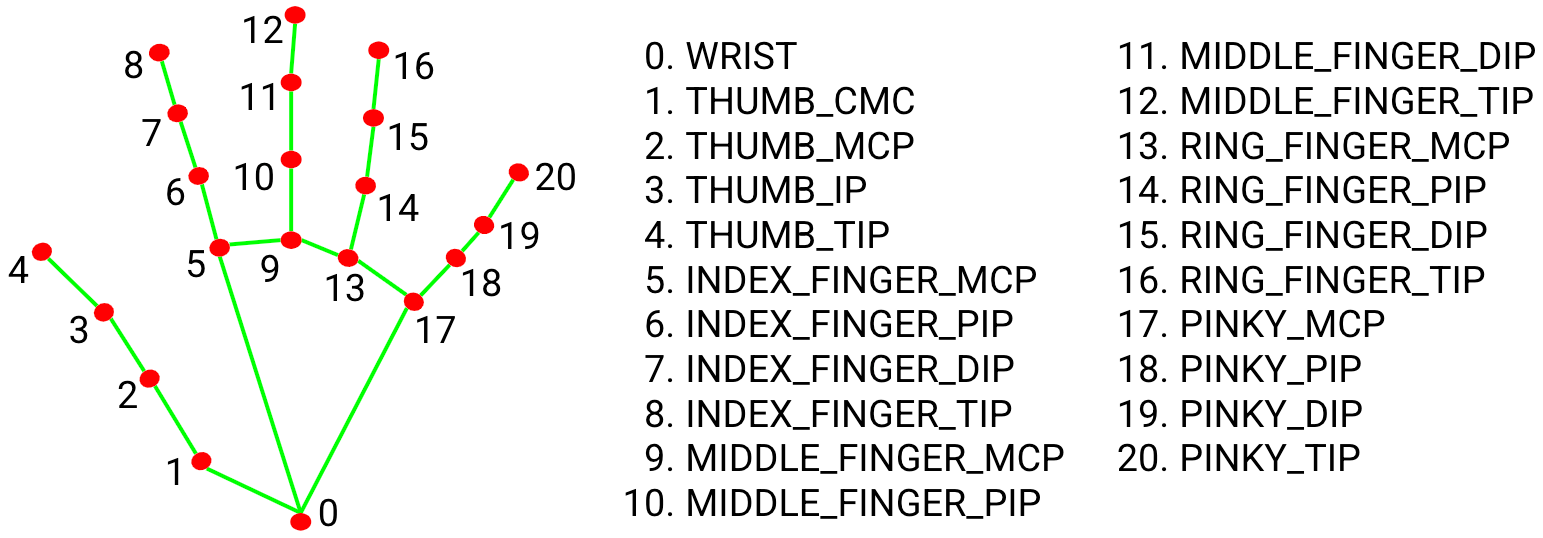
\includegraphics[scale=0.15]{figures/mediapipe_landmarks.png} }}%
    \qquad
    (b) {{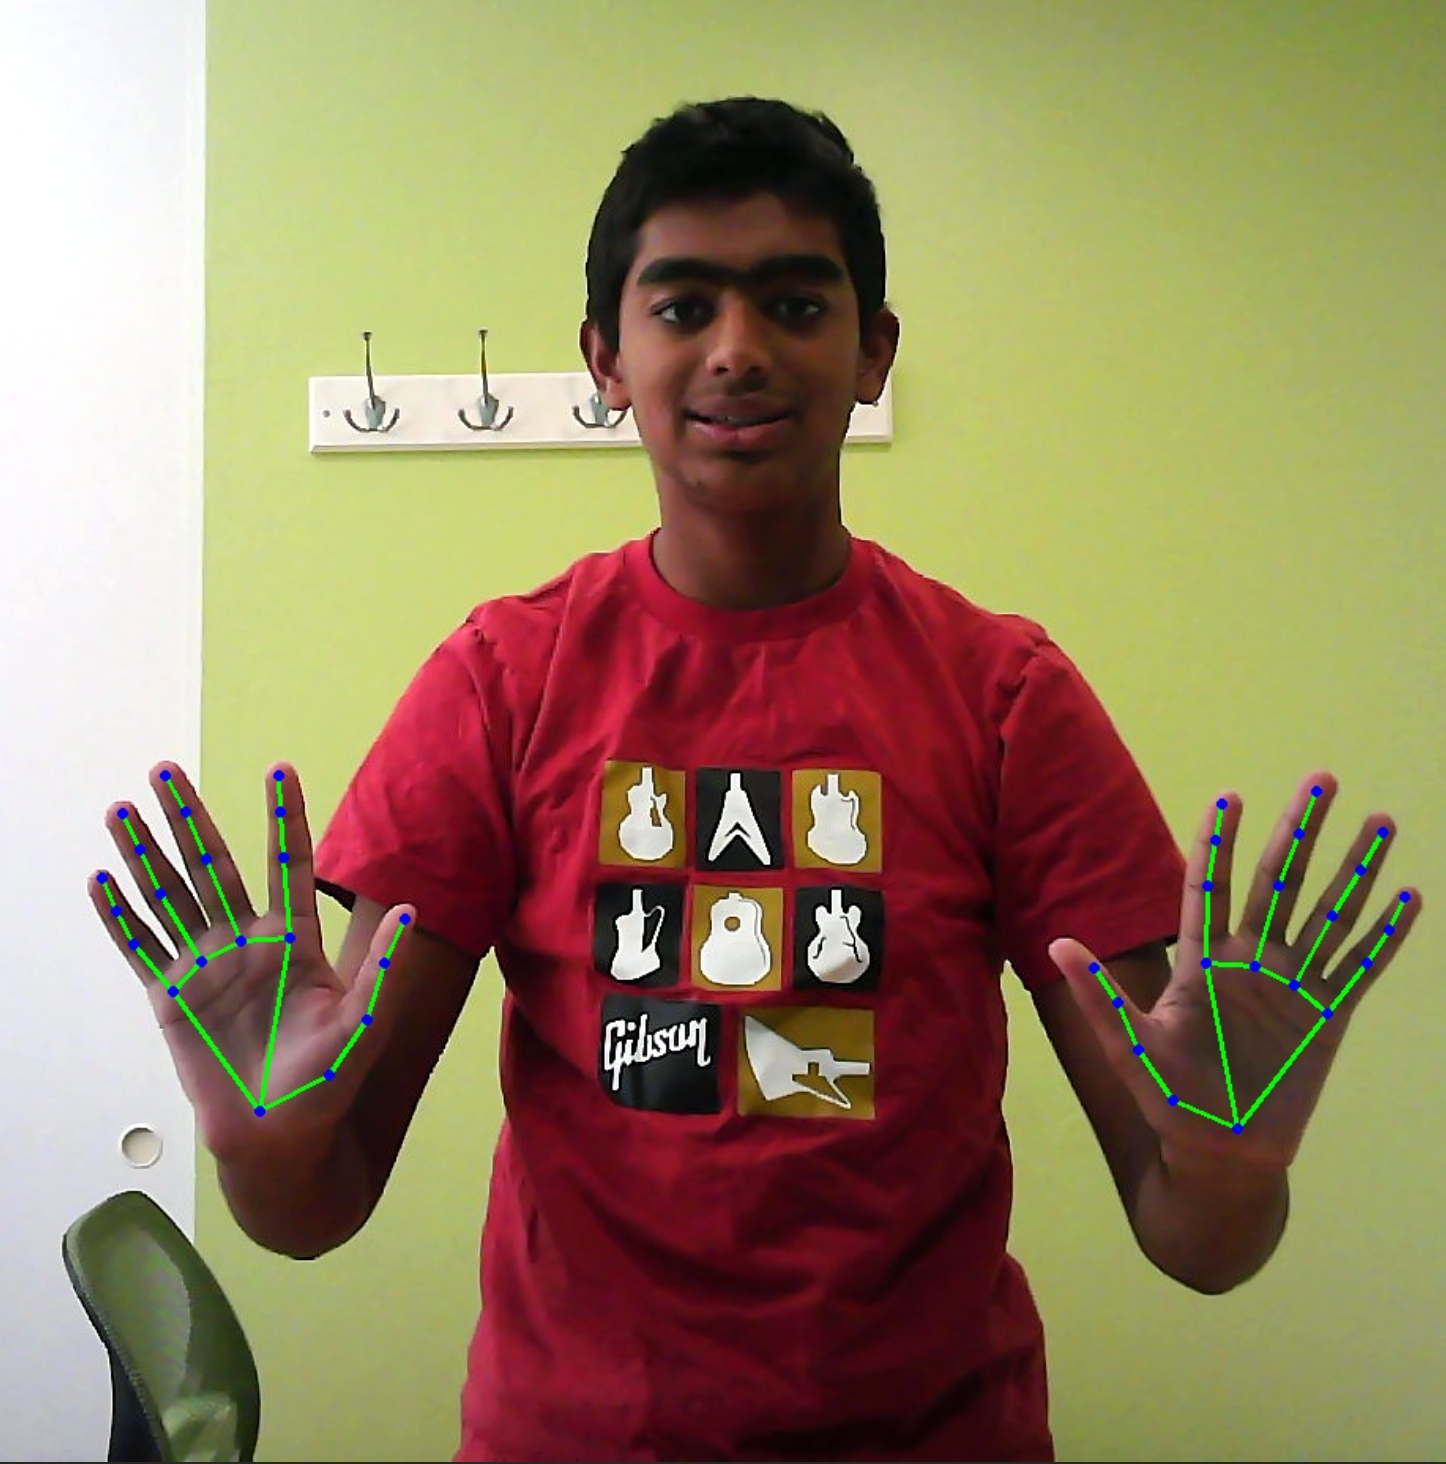
\includegraphics[scale=0.2]{figures/anish_mediapipe.png} }}%
    \caption{Figure 2a shows Mediapipe's detected hand landmarks. Figure 2b shows the drawn detected hand landmarks of an image. }%
    \label{fig:example}%
\end{figure}

Our approach is to take the first 90 frames of a video, and for each frame concatenate the coordinates of a set amount of landmarks into one vector that is then fed as input into an LSTM model. We try with various amounts of landmarks; we first try with all 21 landmarks, then with 6 landmarks, and also with a "mean" landmark. We call all of these approaches "feature approaches." Note that the concatenated coordinates of landmarks will always form a vector that is 6 times larger than the number of landmarks used, because there are 3 coordinates for a single landmark and 2 hands in which the same landmark can be detected. Even with this, our feature representation and model, which we will go into next, is extremely light. 

\subsection{Model Architecture}

Despite using 3 different approaches in the amount of landmarks we use, our model architecture is basically the same throughout. We start of with an LSTM layer with a hidden state of 64. We take the last output of this LSTM and pass it to a fully-connected layer/Dense with a sigmoid activation to get the prediction on whether hand flapping was detected or not, where 0 means no and 1 means yes. To minimize overfitting, we also insert a dropout layer between the LSTM and the Dense layer with a probability of 20\% for dropping out a single output. Our architecture is shown in Table 1. 

\begin{table}[H]
    \centering
    \begin{tabular}{c|c}
    \hline 
    \textbf{Layer} & \textbf{Num. Parameters} \\ 
    \hline 
    LSTM, 64 units & 25856 \\
    \hline
    Dropout, 20\% & 0 \\ 
    \hline
    Dense & 65 \\ 
    \hline
    Sigmoid & 0 \\
    \hline
    \textbf{Total} & \textbf{25, 921} \\ 
    \hline
    \end{tabular}
    \caption{Above shows each of the layers in our model architecture and the number of parameters for each layer. The last row shows the total amount of (trainable) parameters our model has.}
\end{table}

We would like to briefly go over why we choose the architecture we did. We found that adding more than one LSTM or FCNL layer did not make any notable difference in performance; thus we removed it to minimize the model's capacity for overfitting. We also experimented with the output dimensionality of the LSTM, we tried 8, 16, 32, and 64. We found that using 32 and 64 worked about the same; with 64 usually performing slightly better. We experiment with both for all of our feature approaches. 

We also implemented shifting augmentations to prevent from any overfitting that may happen due to the minimal training data. Applying these augmentations on the frames of each video took too long, so we decided to apply these augmentations on the (geometric) location vectors. We applied the same augmentation parameters for all the location frames of the same video; we felt augmenting each location frame individually would create noise that would make it harder for the model to learn. To augment on the width dimension, we make sure find an amount to increase or decrease (equal chance) the \emph{x} coordinates such that no \emph{x} coordinates will be less than 0 or greater than 1 (to keep the data in this range.) \emph{x} coordinates that were 0 before augmentation, meaning they weren't detected, 0 after augmentation. The same method is used for augmenting on the height and depth dimension with the \emph{y} and \emph{z} coordinates respectively. We try all of our feature approaches with and without augmentations. 

We train all of our models with (binary) crossentropy loss and with Adam optimization. We find that the optimal learning rate changes based on the feature approach. All of our models and augmentations are written using TensorFlow and Keras. No GPUs or specialized hardware was ever required; training a single model usually took a few minutes. We show our overall approach in Figure 3. 

\begin{figure}[h!]
\centering
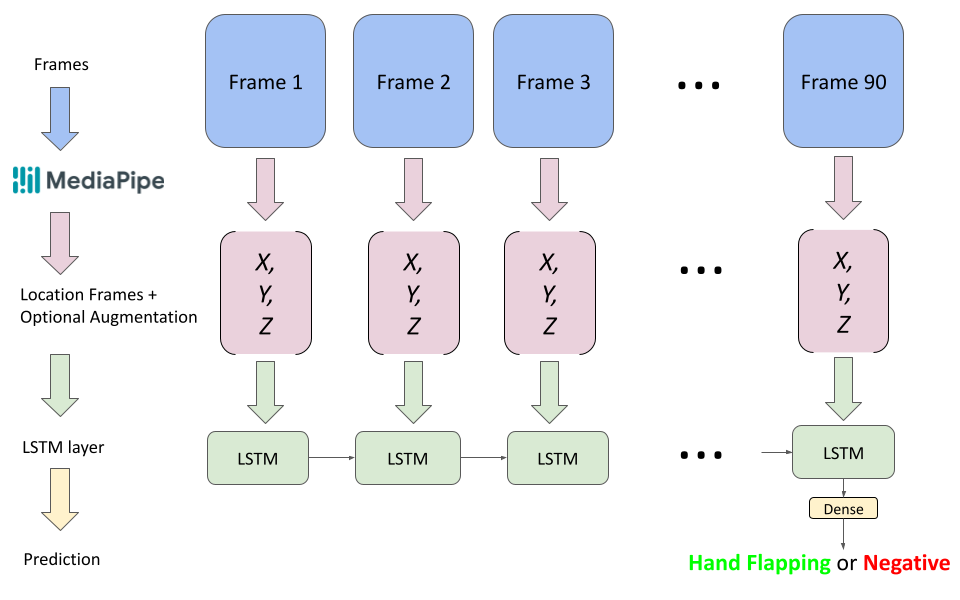
\includegraphics[scale=0.4]{figures/Approach.png}
\caption{Figure to show our overall approach to create a prediction on whether hand flapping was detected.}
\label{fig:method}
\end{figure}

\newpage

\subsection{All Landmarks}

This approach took all of the 21 landmarks on both hands. In order to test how well this model worked, we used 5-fold cross validation. We split up our data into 5 sections, and evaluated our models by training them 5 times - each time on leaving out one fold for validation and training on the rest. We evaluate a model's accuracy, precision, recall, and F1 score on a single run based on the average of the aforementioned metrics across all folds. We run our model, as described in Table 1, ten times and record the mean and standard deviation for each all of the runs' accuracy, precision, recall, and F1 score. The results of our model runs, with and without augmentations, are shown in Table 2. We also show the Receiver Operating Characteristics (ROC) curve and Area under the ROC curve (AUROC) for both models in Figure 4. 

\begin{table}[H]
    \centering
    \begin{tabular}{c|c|c|c|c}
    \hline 
    Model & Classification Accuracy & Precision & Recall & F1 Score \\ 
    \hline 
    Augmentation & 71.2 $\pm$ 2.14 & 69.02 $\pm$ 2.04 & 79.6 $\pm$ 1.29 & 73.22 $\pm$ 1.28 \\
    \hline
    No Augmentation & \textbf{72.4 $\pm$ 0.8} & \textbf{69.68 $\pm$ 0.99} & \textbf{82.92 $\pm$ 0.94} & \textbf{75.15 $\pm$ 0.57} \\ 
    \hline
    \end{tabular}
    \caption{The means and standard deviations of the accuracy, precision, recall, and F1 Score over the 10 runs for both models (one with and one without augmentation) are shown above.}
\end{table}

\begin{figure}[h!]
    \centering
    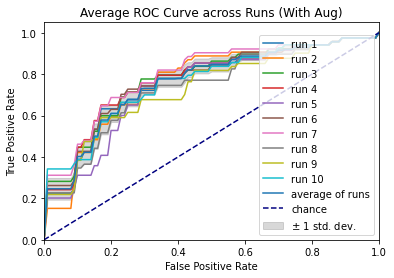
\includegraphics[scale=0.5]{figures/all_landmarks_roc_aug.png}
    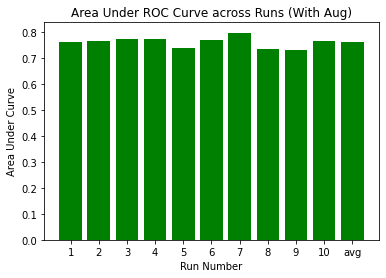
\includegraphics[scale=0.5]{figures/all_landmarks_auroc_aug.png}
    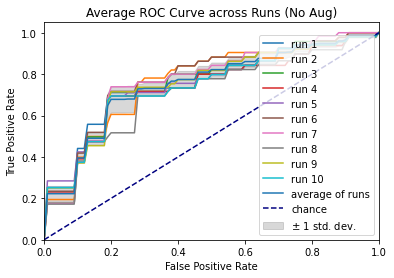
\includegraphics[scale=0.5]{figures/all_landmarks_roc_naug.png}
    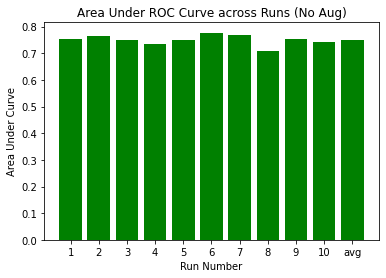
\includegraphics[scale=0.5]{figures/all_landmarks_aurroc_naug.png}
    \caption{Graphs and plots above show the ROC curve and AURROC of both models across all 10 runs. We also show the average of all runs for both models. }
    \label{fig:method}
\end{figure}

The results we achieve with this approach are interesting. The model  without augmentation actually did better than the model with augmentation, by a consistent margin of 0.5-3\% on all metrics. We also note that the model without augmentations achieved more consistent results (less deviation between runs), but this could just be due to the stochastic nature of augmentations. Our best run of a model achieved 74\% classification accuracy, 72\% precision, 82.60\% recall, and an F1 Score of 76.13\%. This model did not use any augmentations. 

While this technique did achieve substantial performance on our dataset, when we applied these models on the 6 hand flapping and control videos we recorded of ourselves the model didn't do as well. 

\subsection{Mean Landmark}
dwadaw
\subsection{Six Landmarks}
dwa

\bibliographystyle{plain}
\bibliography{references.bib}
\end{document}
